% This is "sig-alternate.tex" V2.1 April 2013
% This file should be compiled with V2.5 of "sig-alternate.cls" May 2012
%
% This example file demonstrates the use of the 'sig-alternate.cls'
% V2.5 LaTeX2e document class file. It is for those submitting
% articles to ACM Conference Proceedings WHO DO NOT WISH TO
% STRICTLY ADHERE TO THE SIGS (PUBS-BOARD-ENDORSED) STYLE.
% The 'sig-alternate.cls' file will produce a similar-looking,
% albeit, 'tighter' paper resulting in, invariably, fewer pages.
%
% ----------------------------------------------------------------------------------------------------------------
% This .tex file (and associated .cls V2.5) produces:
%       1) The Permission Statement
%       2) The Conference (location) Info information
%       3) The Copyright Line with ACM data
%       4) NO page numbers
%
% as against the acm_proc_article-sp.cls file which
% DOES NOT produce 1) thru' 3) above.
%
% Using 'sig-alternate.cls' you have control, however, from within
% the source .tex file, over both the CopyrightYear
% (defaulted to 200X) and the ACM Copyright Data
% (defaulted to X-XXXXX-XX-X/XX/XX).
% e.g.
% \CopyrightYear{2007} will cause 2007 to appear in the copyright line.
% \crdata{0-12345-67-8/90/12} will cause 0-12345-67-8/90/12 to appear in the copyright line.
%
% ---------------------------------------------------------------------------------------------------------------
% This .tex source is an example which *does* use
% the .bib file (from which the .bbl file % is produced).
% REMEMBER HOWEVER: After having produced the .bbl file,
% and prior to final submission, you *NEED* to 'insert'
% your .bbl file into your source .tex file so as to provide
% ONE 'self-contained' source file.
%
% ================= IF YOU HAVE QUESTIONS =======================
% Questions regarding the SIGS styles, SIGS policies and
% procedures, Conferences etc. should be sent to
% Adrienne Griscti (griscti@acm.org)
%
% Technical questions _only_ to
% Gerald Murray (murray@hq.acm.org)
% ===============================================================
%
% For tracking purposes - this is V2.0 - May 2012

\documentclass{sig-alternate-05-2015}
\usepackage[T1]{fontenc}
\usepackage{CJKutf8}
\usepackage[english]{babel}

\begin{document}

% Copyright
\setcopyright{acmcopyright}
%\setcopyright{acmlicensed}
%\setcopyright{rightsretained}
%\setcopyright{usgov}
%\setcopyright{usgovmixed}
%\setcopyright{cagov}
%\setcopyright{cagovmixed}


% DOI
\doi{10.475/123_4}

% ISBN
\isbn{123-4567-24-567/08/06}

%Conference
\conferenceinfo{PLDI '13}{June 16--19, 2013, Seattle, WA, USA}

\acmPrice{\$15.00}

%
% --- Author Metadata here ---
\conferenceinfo{WOODSTOCK}{'97 El Paso, Texas USA}
%\CopyrightYear{2007} % Allows default copyright year (20XX) to be over-ridden - IF NEED BE.
%\crdata{0-12345-67-8/90/01}  % Allows default copyright data (0-89791-88-6/97/05) to be over-ridden - IF NEED BE.
% --- End of Author Metadata ---

\title{Alternate {\ttlit ACM} SIG Proceedings Paper in LaTeX
Format\titlenote{(Produces the permission block, and
copyright information). For use with
SIG-ALTERNATE.CLS. Supported by ACM.}}
\subtitle{[Extended Abstract]
\titlenote{A full version of this paper is available as
\textit{Author's Guide to Preparing ACM SIG Proceedings Using
\LaTeX$2_\epsilon$\ and BibTeX} at
\texttt{www.acm.org/eaddress.htm}}}
%
% You need the command \numberofauthors to handle the 'placement
% and alignment' of the authors beneath the title.
%
% For aesthetic reasons, we recommend 'three authors at a time'
% i.e. three 'name/affiliation blocks' be placed beneath the title.
%
% NOTE: You are NOT restricted in how many 'rows' of
% "name/affiliations" may appear. We just ask that you restrict
% the number of 'columns' to three.
%
% Because of the available 'opening page real-estate'
% we ask you to refrain from putting more than six authors
% (two rows with three columns) beneath the article title.
% More than six makes the first-page appear very cluttered indeed.
%
% Use the \alignauthor commands to handle the names
% and affiliations for an 'aesthetic maximum' of six authors.
% Add names, affiliations, addresses for
% the seventh etc. author(s) as the argument for the
% \additionalauthors command.
% These 'additional authors' will be output/set for you
% without further effort on your part as the last section in
% the body of your article BEFORE References or any Appendices.

\numberofauthors{8} %  in this sample file, there are a *total*
% of EIGHT authors. SIX appear on the 'first-page' (for formatting
% reasons) and the remaining two appear in the \additionalauthors section.
%
\author{
% You can go ahead and credit any number of authors here,
% e.g. one 'row of three' or two rows (consisting of one row of three
% and a second row of one, two or three).
%
% The command \alignauthor (no curly braces needed) should
% precede each author name, affiliation/snail-mail address and
% e-mail address. Additionally, tag each line of
% affiliation/address with \affaddr, and tag the
% e-mail address with \email.
%
% 1st. author
\alignauthor
Ben Trovato\titlenote{Dr.~Trovato insisted his name be first.}\\
       \affaddr{Institute for Clarity in Documentation}\\
       \affaddr{1932 Wallamaloo Lane}\\
       \affaddr{Wallamaloo, New Zealand}\\
       \email{trovato@corporation.com}
% 2nd. author
\alignauthor
G.K.M. Tobin\titlenote{The secretary disavows
any knowledge of this author's actions.}\\
       \affaddr{Institute for Clarity in Documentation}\\
       \affaddr{P.O. Box 1212}\\
       \affaddr{Dublin, Ohio 43017-6221}\\
       \email{webmaster@marysville-ohio.com}
% 3rd. author
\alignauthor Lars Th{\o}rv{\"a}ld\titlenote{This author is the
one who did all the really hard work.}\\
       \affaddr{The Th{\o}rv{\"a}ld Group}\\
       \affaddr{1 Th{\o}rv{\"a}ld Circle}\\
       \affaddr{Hekla, Iceland}\\
       \email{larst@affiliation.org}
\and  % use '\and' if you need 'another row' of author names
% 4th. author
\alignauthor Lawrence P. Leipuner\\
       \affaddr{Brookhaven Laboratories}\\
       \affaddr{Brookhaven National Lab}\\
       \affaddr{P.O. Box 5000}\\
       \email{lleipuner@researchlabs.org}
% 5th. author
\alignauthor Sean Fogarty\\
       \affaddr{NASA Ames Research Center}\\
       \affaddr{Moffett Field}\\
       \affaddr{California 94035}\\
       \email{fogartys@amesres.org}
% 6th. author
\alignauthor Charles Palmer\\
       \affaddr{Palmer Research Laboratories}\\
       \affaddr{8600 Datapoint Drive}\\
       \affaddr{San Antonio, Texas 78229}\\
       \email{cpalmer@prl.com}
}
% There's nothing stopping you putting the seventh, eighth, etc.
% author on the opening page (as the 'third row') but we ask,
% for aesthetic reasons that you place these 'additional authors'
% in the \additional authors block, viz.
\additionalauthors{Additional authors: John Smith (The Th{\o}rv{\"a}ld Group,
email: {\texttt{jsmith@affiliation.org}}) and Julius P.~Kumquat
(The Kumquat Consortium, email: {\texttt{jpkumquat@consortium.net}}).}
\date{30 July 1999}
% Just remember to make sure that the TOTAL number of authors
% is the number that will appear on the first page PLUS the
% number that will appear in the \additionalauthors section.

\maketitle
\begin{abstract}
\begin{CJK}{UTF8}{mj}
한글 한글 한글
\end{CJK}
\begin{center}
This paper provides a sample of a \LaTeX\ document which conforms,
somewhat loosely, to the formatting guidelines for
ACM SIG Proceedings. It is an {\em alternate} style which produces
a {\em tighter-looking} paper and was designed in response to
concerns expressed, by authors, over page-budgets.
It complements the document \textit{Author's (Alternate) Guide to
Preparing ACM SIG Proceedings Using \LaTeX$2_\epsilon$\ and Bib\TeX}.
This source file has been written with the intention of being
compiled under \LaTeX$2_\epsilon$\ and BibTeX.

The developers have tried to include every imaginable sort
of ``bells and whistles", such as a subtitle, footnotes on
title, subtitle and authors, as well as in the text, and
every optional component (e.g. Acknowledgments, Additional
Authors, Appendices), not to mention examples of
equations, theorems, tables and figures.

To make best use of this sample document, run it through \LaTeX\
and BibTeX, and compare this source code with the printed
output produced by the dvi file. A compiled PDF version
is available on the web page to help you with the
`look and feel'.
\end{center}
\end{abstract}


%
% The code below should be generated by the tool at
% http://dl.acm.org/ccs.cfm
% Please copy and paste the code instead of the example below. 
%
\begin{CCSXML}
<ccs2012>
 <concept>
  <concept_id>10010520.10010553.10010562</concept_id>
  <concept_desc>Computer systems organization~Embedded systems</concept_desc>
  <concept_significance>500</concept_significance>
 </concept>
 <concept>
  <concept_id>10010520.10010575.10010755</concept_id>
  <concept_desc>Computer systems organization~Redundancy</concept_desc>
  <concept_significance>300</concept_significance>
 </concept>
 <concept>
  <concept_id>10010520.10010553.10010554</concept_id>
  <concept_desc>Computer systems organization~Robotics</concept_desc>
  <concept_significance>100</concept_significance>
 </concept>
 <concept>
  <concept_id>10003033.10003083.10003095</concept_id>
  <concept_desc>Networks~Network reliability</concept_desc>
  <concept_significance>100</concept_significance>
 </concept>
</ccs2012>  
\end{CCSXML}

\ccsdesc[500]{Computer systems organization~Embedded systems}
\ccsdesc[300]{Computer systems organization~Redundancy}
\ccsdesc{Computer systems organization~Robotics}
\ccsdesc[100]{Networks~Network reliability}


%
% End generated code
%

%
%  Use this command to print the description
%
\printccsdesc

% We no longer use \terms command
%\terms{Theory}

\keywords{ACM proceedings; \LaTeX; text tagging}

\section{Introduction}
The \textit{proceedings} are the records of a conference.
ACM seeks to give these conference by-products a uniform,
high-quality appearance.  To do this, ACM has some rigid
requirements for the format of the proceedings documents: there
is a specified format (balanced  double columns), a specified
set of fonts (Arial or Helvetica and Times Roman) in
certain specified sizes (for instance, 9 point for body copy),
a specified live area (18 $\times$ 23.5 cm [7" $\times$ 9.25"]) centered on
the page, specified size of margins (1.9 cm [0.75"]) top, (2.54 cm [1"]) bottom
and (1.9 cm [.75"]) left and right; specified column width
(8.45 cm [3.33"]) and gutter size (.83 cm [.33"]).

The good news is, with only a handful of manual
settings\footnote{Two of these, the {\texttt{\char'134 numberofauthors}}
and {\texttt{\char'134 alignauthor}} commands, you have
already used; another, {\texttt{\char'134 balancecolumns}}, will
be used in your very last run of \LaTeX\ to ensure
balanced column heights on the last page.}, the \LaTeX\ document
class file handles all of this for you.

The remainder of this document is concerned with showing, in
the context of an ``actual'' document, the \LaTeX\ commands
specifically available for denoting the structure of a
proceedings paper, rather than with giving rigorous descriptions
or explanations of such commands.

\section{Solving 8-Puzzle Problem}
\begin{CJK}{UTF8}{mj}
\subsection{Problem}
기존의 유명한 8-퍼즐 문제는 다음과 같다:

<table 1>과 같이 3x3 격자에 1~8의 숫자가 적힌 칸이 하나씩 있고 빈 칸이 하나 있다.
\begin{table}
\centering
\caption{Initial State of 8-Puzzle}
\begin{tabular}{|c|c|c|} \hline
3 & 7 & 1 \\ \hline
6 & 8 & 5 \\ \hline
4 & - & 2 \\ 
\hline\end{tabular}
\end{table}

한 번의 턴은 빈 칸의 상, 하, 좌, 우에 있는 격자 하나를 선택하여 빈 칸으로 움직이는 방식으로 진행된다. 문제는 최소한의 턴으로 <table 2>와 같은 목표 상태를 만들어야 하는 것이다.
\begin{table}
\centering
\caption{Final State of 8-Puzzle}
\begin{tabular}{|c|c|c|} \hline
1 & 2 & 3 \\ \hline
4 & 5 & 6 \\ \hline
7 & 8 & - \\ 
\hline\end{tabular}
\end{table}

본 연구는 기존의 8-퍼즐 문제를 변형한 변형 8-퍼즐 문제를 풀 것이다. 변형 8-퍼즐에서는 빈 칸이 2개 있고 숫자가 1~7까지 있으며 목표 상태는 <table 3>과 같다.
\begin{table}
\centering
\caption{Final State of 8'-Puzzle}
\begin{tabular}{|c|c|c|} \hline
1 & 2 & 3 \\ \hline
- & - & 4 \\ \hline
7 & 6 & 5 \\ 
\hline\end{tabular}
\end{table}
\subsection{Literature Review}
\subsection{Picked Data}
본 연구의 성능 비교는 크게 최악의 경우 성능과 평균 성능을 비교한다. 본 연구에서는 목표 상태를 고정한 후 시작 상태를 랜덤으로 만들어내어 성능을 계산한다.

N개의 시작 상태에 대해서 계산 시간이 $t_1, t_2, ..., t_N$ (ms)인 경우 2000ms 동안 풀 수 있는 퍼즐의 수는 다음과 같이 계산이 가능하다.
\begin{equation} avg = 2000N / \sum_{i=1}^{N}t_i \end{equation}
\begin{equation} worst = 2000 / \max_{i=1}^{N}t_i \end{equation}
\subsection{Algorithm}
본 연구에서 사용할 알고리즘은 A* 알고리즘과 Iterative Deepening Search이다.

Iterative Deepening Search는 깊이를 0에서부터 늘려나가면서 탐색하는 알고리즘이다. 탐색 가능 깊이 0에서부터 점점 깊게 DFS탐색을 하게 하는데, 깊이 i 이하의 노드만 방문할 수 있다. 만약 특정 깊이 t에서 답을 찾는 데 실패한 경우 t를 1씩 늘린 후 DFS탐색을 다시 한다.

A* 알고리즘은 Priority Queue를 이용한 탐색 알고리즘이다. 노드 i에 대해서 현재까지 탐색한 시점에서 시작점에서 노드 i까지의 최단거리를 P(i), 노드 i에서 도착점까지의 예상 최단거리를 Q(i)라고 할 때, P(i)+Q(i)가 가장 작은 노드를 선택해서 그 노드의 다음 노드를 탐색하도록 한다. 함수 Q는 아래와 같은 성질을 만족해야 한다.
\begin{equation} Q(x) \leq dist(x,y) + Q(y) \end{equation}

본 문제에서는 함수 Q를 다음과 같이 설정하였다.
\begin{equation} Q(x) = \sum_{i=1}^{7}{|X_i-Xsol_i| + |Y_i-Ysol_i|} \end{equation}

본 문제는 모든 이동의 비용이 1이므로 $dist(x,y)$는 1이다. 한편, 한 턴을 수행하는 경우 오직 하나의 수만이 위치가 바뀌고 그 수의 맨하탄 거리의 변화량이 많아야 1이므로 $|Q(x)-Q(y)| \le 1$을 만족한다. 따라서 위에서 언급한 함수 Q는 A* 알고리즘에서 사용할 수 있는 함수이다.

\subsection{Experiment}
8-퍼즐을 해결하는 두 가지 알고리즘의 수행속도를 비교하면 <table 4>가 된다.
\begin{table}
\centering
\caption{Performance Analysis of IDS and A*}
\begin{tabular}{|c|c|c|} \hline
Algorithm & Average & Worst \\ \hline
IDS & - & 4 \\ \hline
A* & 6 & 5 \\ 
\hline\end{tabular}
\end{table}

\subsection{Applications}
변형된 8-퍼즐 문제를 해결하는 모든 알고리즘은 정확한 최적해를 구해야 한다. 튜링 머신 상에서 존재하는 문제들 중 많은 문제들이 NP 혹은 그 이상의 문제로 분리되어 현재까지 다항식 꼴의 시간복잡도를 가진 알고리즘이 존재하지 않는다.

따라서 8-퍼즐 문제를 해결하는 데 쓰인 알고리즘은 실제로는 대다수의 NP 문제에서 적용하기 힘들다. A* 알고리즘의 방식과 가장 유사한 알고리즘이 Dijkstra's Shortest Path Algorithm인데, 이 알고리즘에서 A* 알고리즘에서 쓰이는 Q 함수를 새로 정의한다면 방문하는 노드의 수가 평균적으로 더 적어지는 효과를 얻을 수 있다.

따라서 A* 알고리즘의 경우 정보보안 분야에서 활용할 수 있는 범위가 극히 한정적이고 이는 앞에서 설명했듯이 최단경로를 이용한 프로그램의 작은 최적화 수준에 극히 한정된다.

\end{CJK}

\section{KNN Problem}
\begin{CJK}{UTF8}{mj}
\subsection{Problem}
KNN 문제는 두 개의 특성 값과 하나의 분류를 갖고 있는 N개의 표본이 주어질 때, 두 개의 특성 값이 주어지는 새로운 표본이 어떤 분류에 속하는지 구하는 문제이다. 이 문제를 해결하기 위해서 KNN 문제에서는 새로운 표본과 가장 가까운 K개의 표본을 구하여 그 표본들 중에서 가장 많은 표본이 속한 분류를 찾는 방식을 사용한다.
\subsection{Literature Review}
KNN 문제를 해결하는 가장 기본적인 알고리즘은 Brute-force 알고리즘이며, 이 알고리즘은 매우 느리다.
\subsection{Picked Data}
KNN 문제를 테스트하기 위한 데이터는 랜덤 알고리즘을 이용할 것이다. 모든 점에 대해서 $x, y$의 값은 0 이상 100,000 이하의 랜덤한 정수를 사용한다. 분류는 특정 방정식을 만족하는 지에 따라 0 또는 1로 분류할 것이다. 본 연구에서 사용할 방정식은 다음 3개와 같다.
\begin{equation} (y-50000) \geq (x-50000)/2 \end{equation}
\begin{equation} (x-20000)^2 + 2(y-65432)^2 \leq 12345^2 \end{equation}
\begin{equation} (x-2y)(2x-y)(100000-x-y) \geq 0 \end{equation}

알고리즘의 성능 분석은 크게 시간, 정확도 두 가지 측면에서 고려할 것이다. 시간은 2000ms 동안 처리할 수 있는 쿼리의 수를 세며, 정확도는 새로운 표본이 위 3개의 방정식과 일치할 확률을 셀 것이다. 프로그램이 랜덤을 기반으로 하여 실행되지만 수많은 쿼리를 수행하므로 평균은 구할 필요가 없다.
알고리즘을 테스트하기 위해 사용하는 $(N, K)$의 쌍은 <table 5> 와 같다.
\begin{table}
\centering
\caption{Test Vector of (N, K)}
\begin{tabular}{|c|c|c|c|} \hline
N & 1000 & 10000 & 100000 \\ \hline
K & 2 & N/10 & N/2 \\
\hline\end{tabular}
\end{table}

\subsection{Algorithm}
본 문제를 해결하는 데 사용할 알고리즘은 Brute-force 알고리즘과 k-d Tree 알고리즘, 그리고 Locality Sensitive Hashing이다.

Brute-force 알고리즘은 각 쿼리별로 쿼리에 해당하는 점과 가까운 순서대로 N개의 점들을 정렬한 후, 가장 앞선 K개의 표본을 선택하여 답을 구한다. 전처리는 굳이 하지 않으며, 쿼리당 평균 $O(N log N)$의 시간이 걸린다.

k-d Tree 알고리즘은 표본으로 주어진 점들을 가지고 트리를 만든 후, 쿼리로 주어지는 점을 중심으로 하여 K개 의 점을 덮는 원을 잡는다. 이때 k-d Tree를 구성하는 데 $O(N log N)$의 시간이 들며 원 안에 몇 개의 점이 있는지는 k-d Tree 알고리즘을 이용하여 쿼리당 평균 $O(log N)$의 시간으로 구할 수 있다.

Locality Sensitive Hashing 알고리즘에서는 표본으로 주어진 점들을 해싱하여 저장한 뒤, 쿼리로 주어지는 점들에 대해서 그 점의 해시 값을 구한 후 그 값 주변의 해시 값을 가진 점들을 K개 고른다. 여기서 해싱 알고리즘은 Locality Sensitive Hashing이라는 특수한 알고리즘을 사용하는데, Locality Sensitive Hashing은 상수 $R, cR, P_1, P_2$에 대해서 다음 두 식을 만족해야 한다.
\begin{equation} P(h(p)=h(q) | dist(p,q) \leq R) \geq P_1 \end{equation}
\begin{equation} P(h(p)=h(q) | dist(p,q) \geq cR) \leq P_2 \end{equation}
본 연구에서는 Bit Sampling Algorithm\cite{bowman:reasoning, clark:pct, braams:babel,	 herlihy:methodology}을 응용한 방법을 사용한다.
\subsection{Experiment}
\subsubsection{Comparison with Performance}
각 유형 및 N의 크기별로 각 알고리즘의 수행시간을 비교한 결과 <table 6, 7, 8>과 같다.
\begin{table}
\centering
\caption{Performance of Brute-Force, K = 2}
\begin{tabular}{|c|c|c|c|} \hline
N & type 1 & type 2 & type 3 \\ \hline
1000 & 5858 & 5647 & 5808 \\ \hline
10000 & 434 & 433 & 434 \\ \hline
100000 & 29 & 30 & 30 \\ 
\hline\end{tabular}
\end{table}

\begin{table}
\centering
\caption{Performance of K-d Tree, K = 2}
\begin{tabular}{|c|c|c|c|} \hline
N & type 1 & type 2 & type 3 \\ \hline
1000 & 17593 & 17853 & 17582 \\ \hline
10000 & 2220 & 2244 & 2271 \\ \hline
100000 & 196 & 193 & 196 \\ 
\hline\end{tabular}
\end{table}

\begin{table}
\centering
\caption{Performance of LSH, K = 2}
\begin{tabular}{|c|c|c|c|} \hline
N & type 1 & type 2 & type 3 \\ \hline
1000 & 939493 & 953135 & 981269 \\ \hline
10000 & 2123155 & 2223631 & 2071188 \\ \hline
100000 & 2044423 & 2134503 & 1992939 \\ 
\hline\end{tabular}
\end{table}

그 결과, 전체적인 성능은 Brute-force < K-d Tree < LSH 순서대로 나타났으며, Brute-force와 K-d Tree의 경우 N이 커질수록 처리할 수 있는 쿼리의 수는 줄어드는 경향이 나타났고 LSH의 경우 N이 커지면 오히려 처리할 수 있는 쿼리가 많아졌다. 이는 Brute-force와 K-d Tree는 쿼리의 처리시간이 N에 비례하지만 LSH의 경우 쿼리의 처리시간이 주어진 정보의 밀도에 반비례하기 때문이다. 반면, 점들의 분포 별 성능은 유의미한 차이를 보이지 않았다.

K의 크기별로 각 알고리즘의 수행 속도를 비교한 결과 <table 9>와 같다.

\begin{table}
\centering
\caption{Performance by K, N = 10000, type 3}
\begin{tabular}{|c|c|c|c|} \hline
Algorithm & K=2 & K=1000 & K=5000 \\ \hline
Brute-force & 428 & 432 & 424 \\ \hline
K-d Tree & 2278 & 1779 & 1143 \\ \hline
LSH & 2107781 & 18180 & 3745 \\ 
\hline\end{tabular}
\end{table}

전체적인 성능은 K-d Tree와 LSH 알고리즘에서 $K=2$ < $K=1000$ < $K=5000$ 의 경향을 띄고 Brute-force 알고리즘은 성능이 K에 관련이 없는 것과 같이 보인다. Brute-force의 경우 쿼리의 수행시간이 $N logN + K$인데, K가 $N log N$에 비해 매우 작기 때문이다. K-d Tree에서 K가 커질 때 수행시간이 느려지는 이유는 원의 크기가 커져서 고려해야 할 K-d Tree의 노드의 수가 많기 때문이다. LSH 알고리즘에서는 수행시간이 많이 느려지는데, 이는 쿼리 별 시간복잡도가 O(K)이기 때문으로 보인다.

\subsubsection{Comparison with Accuracy}
각 유형 및 N의 크기별로 각 알고리즘의 수행 정확도를 비교한 결과 <table 10, 11, 12>와 같다.
\begin{table}
\centering
\caption{Accuracy of Brute-Force, K = 2}
\begin{tabular}{|c|c|c|c|} \hline
N & type 1 & type 2 & type 3 \\ \hline
1000 & 0.987026 & 0.994791 & 0.954718 \\ \hline
10000 & 0.993088 & 0.995381 & 0.972350 \\ \hline
100000 & 1.000000 & 1.000000 & 1.000000 \\ 
\hline\end{tabular}
\end{table}

\begin{table}
\centering
\caption{Accuracy of K-d Tree, K = 2}
\begin{tabular}{|c|c|c|c|} \hline
N & type 1 & type 2 & type 3 \\ \hline
1000 & 0.986699 & 0.994791 & 0.954897 \\ \hline
10000 & 0.991892 & 0.998217 & 0.985909 \\ \hline
100000 & 1.000000 & 1.000000 & 1.000000 \\ 
\hline\end{tabular}
\end{table}

\begin{table}
\centering
\caption{Accuracy of LSH, K = 2}
\begin{tabular}{|c|c|c|c|} \hline
N & type 1 & type 2 & type 3 \\ \hline
1000 & 0.546098 & 0.966076 & 0.519885 \\ \hline
10000 & 0.543720 & 0.964420 & 0.528809 \\ \hline
100000 & 0.548303 & 0.964482 & 0.530148 \\ 
\hline\end{tabular}
\end{table}

그 결과, 전체적인 성능은 LSH < K-d Tree = Brute-force 순서대로 나타났다. 이는 K-d Tree와 Brute-force 알고리즘은 결정론적인 알고리즘이지만 LSH는 랜덤을 이용한 알고리즘이기 때문에 일어나는 현상이다. 한편  LSH의 경우 점들의 분포에 따라 알고리즘의 정확성에 큰 차이를 보였다. 이는 type 1과 type 3에 비해 type 2가 x와 y의 차이가 작아서 해시 함수의 값의 분포가 좁기 때문으로 보인다. 반면, N의 크기와 성능은 유의미한 차이를 보이지 않았다.

K의 크기별로 각 알고리즘의 수행 정확도를 비교한 결과 table D와 같다.

\begin{table}
\centering
\caption{Accuracy by K, N = 10000, type 3}
\begin{tabular}{|c|c|c|c|} \hline
Algorithm & K=2 & K=1000 & K=5000 \\ \hline
Brute-force & 0.971963 & 0.923611 & 0.648585 \\ \hline
K-d Tree & 0.985963 & 0.978078 & 0.948381 \\ \hline
LSH & 0.528441 & 0.676898 & 0.647797 \\ 
\hline\end{tabular}
\end{table}

Brute-force 알고리즘과 K-d Tree에서는 $K=2$ > $K=1000$ > $K=5000$ 순으로 정확도가 나타났다. 실제로 고려하는 점의 수가 많은 경우에는 상대적으로 쿼리로 주어진 점에서 먼 점을 보기 때문에 분류를 잘못 선택할 확률이 높아진다. Brute-force 알고리즘에서 $K=5000$일 때 정확도가 급격히 떨어진 데 비해 K-d Tree 알고리즘에서 정확도의 차이가 적은데, 이는 K-d Tree 알고리즘에서 5000개보다 약간 더 많은 노드를 보기 때문이다. LSH 알고리즘에서는 $K=1000$ > $K=5000$ > $K=2$ 순으로 정확도가 나타났는데, 이는 쿼리로 주어진 점과 가까운 점을 많이 포함시키기 위해서 K가 적당히 클 필요가 있기 때문이다.

\subsection{Applications}
\end{CJK}

\section{Map Coloring Problem}
\begin{CJK}{UTF8}{mj}
\subsection{Problem}
지도 색칠 문제는 지도를 색칠하는 문제로 
\subsection{Literature Review}
\subsection{Picked Data}
\subsection{Algorithm}
본 연구에서 사용할 알고리즘은 A* 알고리즘과 Iterative Deepening Search이다.
Iterative Deepening Search는 깊이를 1에서부터 늘려나가면서 탐색하는 알고리즘이다.
\subsection{Experiment}
\subsection{Applications}
\end{CJK}

\section{Sequence Guessing Problem}
\begin{CJK}{UTF8}{mj}
\subsection{Problem}
수열 예측 문제는 수열 ${A_n}$의 첫 N개의 항 $A_1, A_2, ..., A_N$이 주어질 때 그 이후의 항들을 예측하는 문제이다.

본 연구에서는 우선 기존의 유명한 수열들을 가지고 항들을 예측한 후, 이를 이용하여 대한민국의 1970~2016년 GDP를 이용하여 2017년~2025년의 GDP를 예측할 것이다.

\subsection{Literature Review}
본 문제를 해결하기 위해 처음에는 Linear Regression을 이용하여 Minimum Square Sum을 유도하였다. 그러나 선형 관계가 아닌 경우 Linear Regression은 한계가 발생하였다.

이를 해결하기 위하여 등장한 알고리즘은 Gaussian Process Regression (GPR)을 활용한 알고리즘이다.
GPR은 특정 ${(x_i,y_i) | 1<=i<=N}$에 대해서 $y = f(x)$를 만족하는 f를 예측하는 알고리즘이다. 실제로는 f를 예측하는 것이 매우 어려우므로 특정 x'에 대해서 $y' = f(x')$ 를 만족하는 y'의 값을 예측할 것이다.

Gaussian Noise Model을 생각해보자.

$y = f(x) + N(0, \sigma_n^2)$

Gaussian Process는 Random Process로 다음 조건을 만족한다.

\begin{equation} E(G(x)) = 0 \end{equation}
\begin{equation} k(G(x),G(x')) = \sigma_f^2 exp({-(x-x')^2} over {2l^2}) \end{equation}

우리는 수열을 볼 때 y = f(x) + 

\subsection{Picked Data}
본 연구에서는 특정한 여러 종류의 수열에 대해서 N의 값을 조절해가며 그 이후의 K개 항의 오차를 계산할 것이다.

우선 모든 실험에서 $\sigma_n$을 1로 고정시킨다. 그 후 본 연구에서는 다양한 변인들을 통제하며 GDP 예측에 가장 적합한 방법을 찾을 것이다.

- N, K를 늘려가면서 오차를 계산

- 기존 수열을 여러 가지 형태로 바꾸어 계산

- $\sigma_f, l$ 을 구하는 알고리즘에 따른 분석

- 오차 측정 알고리즘에 따른 분석

특히, 수열을 여러 가지 형태로 바꾸어 계산하는 경우 선형 점화식을 가진 수열과 그렇지 않은 수열 몇 개를 선정하여 분석할 것이다. 선형 점화식을 가진 수열은 대표적으로 아래와 같다.
\begin{equation} f(x) = x \end{equation}
\begin{equation} f(x) = x^2 \end{equation}
\begin{equation} f(0)=0, f(1)=1, f(i+2)=f(i+1)+f(i) \end{equation}

그렇지 않은 수열은 대표적으로 아래와 같다.
\begin{equation} f(x) = 100 sin{x} \end{equation}
\begin{equation} f(x) = 100/x \end{equation}


\subsection{Algorithm}
GPR 알고리즘에서 가장 중요한 것은 $\sigma_n$ 을 고정시키고 $\sigma_f, l$ 를 변화시키는 것이다. 가장 알맞은 $\sigma_f, l$을 구하여 오차를 최소한으로 줄이기 위해서는 오차 측정 알고리즘과 $\sigma_f, l$를 선정하는 알고리즘 두 개를 만들어야 한다.

$\sigma_f, l$을 구하는 알고리즘은 세 가지 있는데 모두 비슷한 부류의 Brute-force 알고리즘이다.

- $\sigma_f, l$을 모두 1~25 범위에서 Brute-force 검색

- l을 15로 고정시켜 놓은 후  $\sigma_f$를 1~700 범위에서 Brute-force 검색

- 백의 자리, 십의 자리, 일의 자리 순서대로 가장 적절한 $\sigma_f, l$를 쌓기

가장 알맞은 $\sigma_f, l$이 되기 위한 조건은 Sum of Error Square을 최소화시키는 것이다.

\begin{equation} E(G(x)) = 0 \end{equation}

\subsection{Experiment}
\subsection{Applications}
\end{CJK}

\section{Number Reading Problem}
\begin{CJK}{UTF8}{mj}
\subsection{Problem}
숫자 인식 문제는 28 x 28 크기의 이미지가 주어지면 그 이미지에 그려진 숫자를 판별하는 문제이다.
\subsection{Literature Review}
\subsection{Picked Data}
본 문제에서는 MNIST의 데이터베이스를 이용하여 학습 및 테스트를 할 것이다.
\subsection{Algorithm}
본 연구에서 사용할 알고리즘은 Tensorflow를 사용한 Artifitial Neural Network 알고리즘이다.
\subsection{Experiment}
\subsection{Applications}
\end{CJK}

\section{The {\secit Body} of The Paper}
Typically, the body of a paper is organized
into a hierarchical structure, with numbered or unnumbered
headings for sections, subsections, sub-subsections, and even
smaller sections.  The command \texttt{{\char'134}section} that
precedes this paragraph is part of such a
hierarchy.\footnote{This is the second footnote.  It
starts a series of three footnotes that add nothing
informational, but just give an idea of how footnotes work
and look. It is a wordy one, just so you see
how a longish one plays out.} \LaTeX\ handles the numbering
and placement of these headings for you, when you use
the appropriate heading commands around the titles
of the headings.  If you want a sub-subsection or
smaller part to be unnumbered in your output, simply append an
asterisk to the command name.  Examples of both
numbered and unnumbered headings will appear throughout the
balance of this sample document.

Because the entire article is contained in
the \textbf{document} environment, you can indicate the
start of a new paragraph with a blank line in your
input file; that is why this sentence forms a separate paragraph.

\subsection{Type Changes and {\subsecit Special} Characters}
We have already seen several typeface changes in this sample.  You
can indicate italicized words or phrases in your text with
the command \texttt{{\char'134}textit}; emboldening with the
command \texttt{{\char'134}textbf}
and typewriter-style (for instance, for computer code) with
\texttt{{\char'134}texttt}.  But remember, you do not
have to indicate typestyle changes when such changes are
part of the \textit{structural} elements of your
article; for instance, the heading of this subsection will
be in a sans serif\footnote{A third footnote, here.
Let's make this a rather short one to
see how it looks.} typeface, but that is handled by the
document class file. Take care with the use
of\footnote{A fourth, and last, footnote.}
the curly braces in typeface changes; they mark
the beginning and end of
the text that is to be in the different typeface.

You can use whatever symbols, accented characters, or
non-English characters you need anywhere in your document;
you can find a complete list of what is
available in the \textit{\LaTeX\
User's Guide}\cite{Lamport:LaTeX}.

\subsection{Math Equations}
You may want to display math equations in three distinct styles:
inline, numbered or non-numbered display.  Each of
the three are discussed in the next sections.

\subsubsection{Inline (In-text) Equations}
A formula that appears in the running text is called an
inline or in-text formula.  It is produced by the
\textbf{math} environment, which can be
invoked with the usual \texttt{{\char'134}begin. . .{\char'134}end}
construction or with the short form \texttt{\$. . .\$}. You
can use any of the symbols and structures,
from $\alpha$ to $\omega$, available in
\LaTeX\cite{Lamport:LaTeX}; this section will simply show a
few examples of in-text equations in context. Notice how
this equation: \begin{math}\lim_{n\rightarrow \infty}x=0\end{math},
set here in in-line math style, looks slightly different when
set in display style.  (See next section).

\subsubsection{Display Equations}
A numbered display equation -- one set off by vertical space
from the text and centered horizontally -- is produced
by the \textbf{equation} environment. An unnumbered display
equation is produced by the \textbf{displaymath} environment.

Again, in either environment, you can use any of the symbols
and structures available in \LaTeX; this section will just
give a couple of examples of display equations in context.
First, consider the equation, shown as an inline equation above:
\begin{equation}\lim_{n\rightarrow \infty}x=0\end{equation}
Notice how it is formatted somewhat differently in
the \textbf{displaymath}
environment.  Now, we'll enter an unnumbered equation:
\begin{displaymath}\sum_{i=0}^{\infty} x + 1\end{displaymath}
and follow it with another numbered equation:
\begin{equation}\sum_{i=0}^{\infty}x_i=\int_{0}^{\pi+2} f\end{equation}
just to demonstrate \LaTeX's able handling of numbering.

\subsection{Citations}
Citations to articles \cite{bowman:reasoning,
clark:pct, braams:babel, herlihy:methodology},
conference proceedings \cite{clark:pct} or
books \cite{salas:calculus, Lamport:LaTeX} listed
in the Bibliography section of your
article will occur throughout the text of your article.
You should use BibTeX to automatically produce this bibliography;
you simply need to insert one of several citation commands with
a key of the item cited in the proper location in
the \texttt{.tex} file \cite{Lamport:LaTeX}.
The key is a short reference you invent to uniquely
identify each work; in this sample document, the key is
the first author's surname and a
word from the title.  This identifying key is included
with each item in the \texttt{.bib} file for your article.

The details of the construction of the \texttt{.bib} file
are beyond the scope of this sample document, but more
information can be found in the \textit{Author's Guide},
and exhaustive details in the \textit{\LaTeX\ User's
Guide}\cite{Lamport:LaTeX}.

This article shows only the plainest form
of the citation command, using \texttt{{\char'134}cite}.
This is what is stipulated in the SIGS style specifications.
No other citation format is endorsed or supported.

\subsection{Tables}
Because tables cannot be split across pages, the best
placement for them is typically the top of the page
nearest their initial cite.  To
ensure this proper ``floating'' placement of tables, use the
environment \textbf{table} to enclose the table's contents and
the table caption.  The contents of the table itself must go
in the \textbf{tabular} environment, to
be aligned properly in rows and columns, with the desired
horizontal and vertical rules.  Again, detailed instructions
on \textbf{tabular} material
is found in the \textit{\LaTeX\ User's Guide}.

Immediately following this sentence is the point at which
Table 1 is included in the input file; compare the
placement of the table here with the table in the printed
dvi output of this document.

\begin{table}
\centering
\caption{Frequency of Special Characters}
\begin{tabular}{|c|c|l|} \hline
Non-English or Math&Frequency&Comments\\ \hline
\O & 1 in 1,000& For Swedish names\\ \hline
$\pi$ & 1 in 5& Common in math\\ \hline
\$ & 4 in 5 & Used in business\\ \hline
$\Psi^2_1$ & 1 in 40,000& Unexplained usage\\
\hline\end{tabular}
\end{table}

To set a wider table, which takes up the whole width of
the page's live area, use the environment
\textbf{table*} to enclose the table's contents and
the table caption.  As with a single-column table, this wide
table will ``float" to a location deemed more desirable.
Immediately following this sentence is the point at which
Table 2 is included in the input file; again, it is
instructive to compare the placement of the
table here with the table in the printed dvi
output of this document.


\begin{table*}
\centering
\caption{Some Typical Commands}
\begin{tabular}{|c|c|l|} \hline
Command&A Number&Comments\\ \hline
\texttt{{\char'134}alignauthor} & 100& Author alignment\\ \hline
\texttt{{\char'134}numberofauthors}& 200& Author enumeration\\ \hline
\texttt{{\char'134}table}& 300 & For tables\\ \hline
\texttt{{\char'134}table*}& 400& For wider tables\\ \hline\end{tabular}
\end{table*}
% end the environment with {table*}, NOTE not {table}!

\subsection{Figures}
Like tables, figures cannot be split across pages; the
best placement for them
is typically the top or the bottom of the page nearest
their initial cite.  To ensure this proper ``floating'' placement
of figures, use the environment
\textbf{figure} to enclose the figure and its caption.

This sample document contains examples of \textbf{.eps} files to be
displayable with \LaTeX.  If you work with pdf\LaTeX, use files in the
\textbf{.pdf} format.  Note that most modern \TeX\ system will convert
\textbf{.eps} to \textbf{.pdf} for you on the fly.  More details on
each of these is found in the \textit{Author's Guide}.

\begin{figure}
\centering
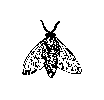
\includegraphics{fly}
\caption{A sample black and white graphic.}
\end{figure}

\begin{figure}
\centering
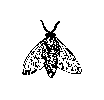
\includegraphics[height=1in, width=1in]{fly}
\caption{A sample black and white graphic
that has been resized with the \texttt{includegraphics} command.}
\end{figure}


As was the case with tables, you may want a figure
that spans two columns.  To do this, and still to
ensure proper ``floating'' placement of tables, use the environment
\textbf{figure*} to enclose the figure and its caption.
and don't forget to end the environment with
{figure*}, not {figure}!

\begin{figure*}
\centering
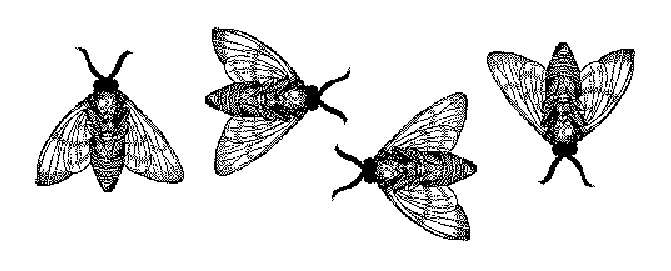
\includegraphics{flies}
\caption{A sample black and white graphic
that needs to span two columns of text.}
\end{figure*}


\begin{figure}
\centering
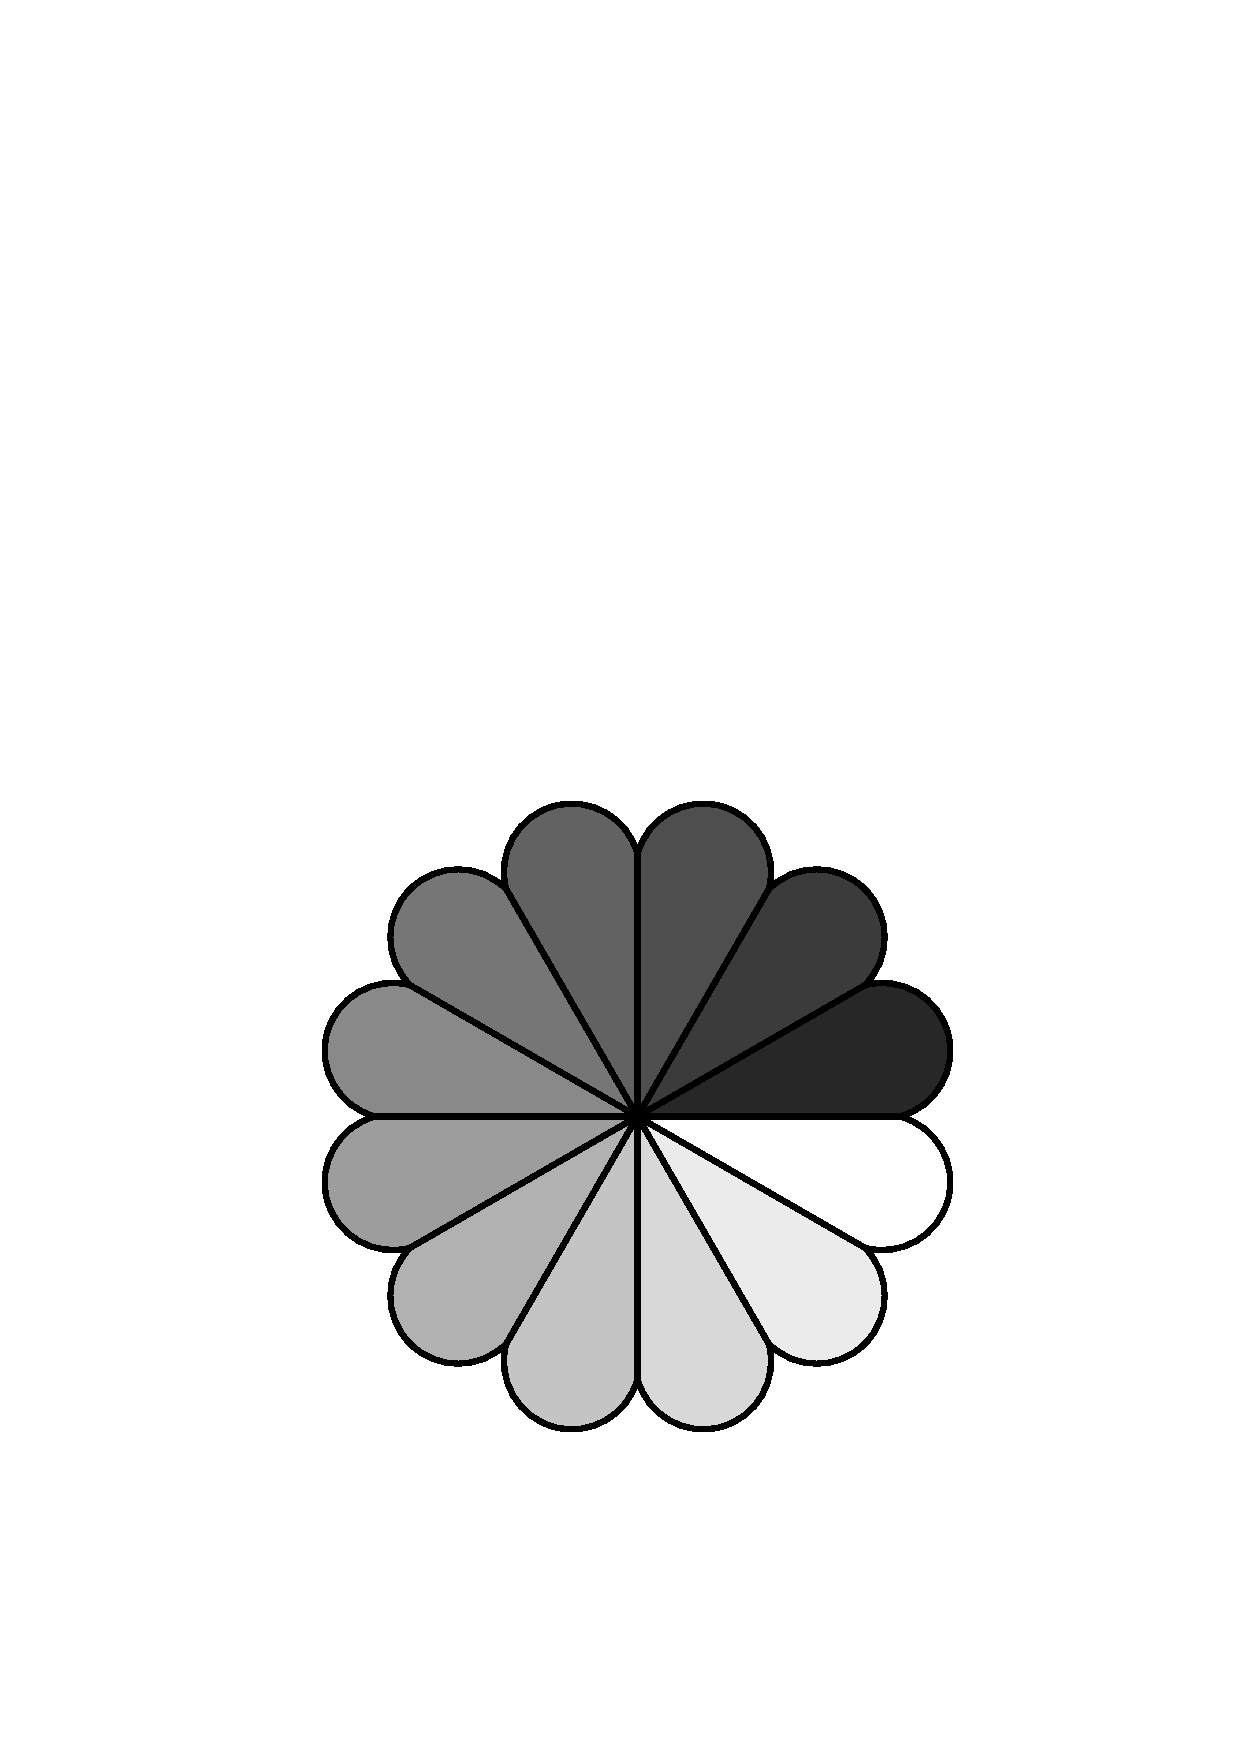
\includegraphics[height=1in, width=1in]{rosette}
\caption{A sample black and white graphic that has
been resized with the \texttt{includegraphics} command.}
\vskip -6pt
\end{figure}

\subsection{Theorem-like Constructs}
Other common constructs that may occur in your article are
the forms for logical constructs like theorems, axioms,
corollaries and proofs.  There are
two forms, one produced by the
command \texttt{{\char'134}newtheorem} and the
other by the command \texttt{{\char'134}newdef}; perhaps
the clearest and easiest way to distinguish them is
to compare the two in the output of this sample document:

This uses the \textbf{theorem} environment, created by
the\linebreak\texttt{{\char'134}newtheorem} command:
\newtheorem{theorem}{Theorem}
\begin{theorem}
Let $f$ be continuous on $[a,b]$.  If $G$ is
an antiderivative for $f$ on $[a,b]$, then
\begin{displaymath}\int^b_af(t)dt = G(b) - G(a).\end{displaymath}
\end{theorem}

The other uses the \textbf{definition} environment, created
by the \texttt{{\char'134}newdef} command:
\newdef{definition}{Definition}
\begin{definition}
If $z$ is irrational, then by $e^z$ we mean the
unique number which has
logarithm $z$: \begin{displaymath}{\log e^z = z}\end{displaymath}
\end{definition}

Two lists of constructs that use one of these
forms is given in the
\textit{Author's  Guidelines}.
 
There is one other similar construct environment, which is
already set up
for you; i.e. you must \textit{not} use
a \texttt{{\char'134}newdef} command to
create it: the \textbf{proof} environment.  Here
is a example of its use:
\begin{proof}
Suppose on the contrary there exists a real number $L$ such that
\begin{displaymath}
\lim_{x\rightarrow\infty} \frac{f(x)}{g(x)} = L.
\end{displaymath}
Then
\begin{displaymath}
l=\lim_{x\rightarrow c} f(x)
= \lim_{x\rightarrow c}
\left[ g{x} \cdot \frac{f(x)}{g(x)} \right ]
= \lim_{x\rightarrow c} g(x) \cdot \lim_{x\rightarrow c}
\frac{f(x)}{g(x)} = 0\cdot L = 0,
\end{displaymath}
which contradicts our assumption that $l\neq 0$.
\end{proof}

Complete rules about using these environments and using the
two different creation commands are in the
\textit{Author's Guide}; please consult it for more
detailed instructions.  If you need to use another construct,
not listed therein, which you want to have the same
formatting as the Theorem
or the Definition\cite{salas:calculus} shown above,
use the \texttt{{\char'134}newtheorem} or the
\texttt{{\char'134}newdef} command,
respectively, to create it.

\subsection*{A {\secit Caveat} for the \TeX\ Expert}
Because you have just been given permission to
use the \texttt{{\char'134}newdef} command to create a
new form, you might think you can
use \TeX's \texttt{{\char'134}def} to create a
new command: \textit{Please refrain from doing this!}
Remember that your \LaTeX\ source code is primarily intended
to create camera-ready copy, but may be converted
to other forms -- e.g. HTML. If you inadvertently omit
some or all of the \texttt{{\char'134}def}s recompilation will
be, to say the least, problematic.

\section{Conclusions}
This paragraph will end the body of this sample document.
Remember that you might still have Acknowledgments or
Appendices; brief samples of these
follow.  There is still the Bibliography to deal with; and
we will make a disclaimer about that here: with the exception
of the reference to the \LaTeX\ book, the citations in
this paper are to articles which have nothing to
do with the present subject and are used as
examples only.
%\end{document}  % This is where a 'short' article might terminate

%ACKNOWLEDGMENTS are optional
\section{Acknowledgments}
This section is optional; it is a location for you
to acknowledge grants, funding, editing assistance and
what have you.  In the present case, for example, the
authors would like to thank Gerald Murray of ACM for
his help in codifying this \textit{Author's Guide}
and the \textbf{.cls} and \textbf{.tex} files that it describes.

%
% The following two commands are all you need in the
% initial runs of your .tex file to
% produce the bibliography for the citations in your paper.
\bibliographystyle{abbrv}
\bibliography{sigproc}  % sigproc.bib is the name of the Bibliography in this case
% You must have a proper ".bib" file
%  and remember to run:
% latex bibtex latex latex
% to resolve all references
%
% ACM needs 'a single self-contained file'!
%
%APPENDICES are optional
%\balancecolumns
\appendix
%Appendix A
\section{Headings in Appendices}
The rules about hierarchical headings discussed above for
the body of the article are different in the appendices.
In the \textbf{appendix} environment, the command
\textbf{section} is used to
indicate the start of each Appendix, with alphabetic order
designation (i.e. the first is A, the second B, etc.) and
a title (if you include one).  So, if you need
hierarchical structure
\textit{within} an Appendix, start with \textbf{subsection} as the
highest level. Here is an outline of the body of this
document in Appendix-appropriate form:
\subsection{Introduction}
\subsection{The Body of the Paper}
\subsubsection{Type Changes and  Special Characters}
\subsubsection{Math Equations}
\paragraph{Inline (In-text) Equations}
\paragraph{Display Equations}
\subsubsection{Citations}
\subsubsection{Tables}
\subsubsection{Figures}
\subsubsection{Theorem-like Constructs}
\subsubsection*{A Caveat for the \TeX\ Expert}
\subsection{Conclusions}
\subsection{Acknowledgments}
\subsection{Additional Authors}
This section is inserted by \LaTeX; you do not insert it.
You just add the names and information in the
\texttt{{\char'134}additionalauthors} command at the start
of the document.
\subsection{References}
Generated by bibtex from your ~.bib file.  Run latex,
then bibtex, then latex twice (to resolve references)
to create the ~.bbl file.  Insert that ~.bbl file into
the .tex source file and comment out
the command \texttt{{\char'134}thebibliography}.
% This next section command marks the start of
% Appendix B, and does not continue the present hierarchy
\section{More Help for the Hardy}
The sig-alternate.cls file itself is chock-full of succinct
and helpful comments.  If you consider yourself a moderately
experienced to expert user of \LaTeX, you may find reading
it useful but please remember not to change it.
%\balancecolumns % GM June 2007
% That's all folks!
\end{document}
